\documentclass[tikz,border=12pt]{standalone}
% Shared UMM figure style (journal-consistent palette + line weights)
\usepackage{tikz}
\usepackage{pgfplots}
\pgfplotsset{compat=1.18}
\usetikzlibrary{arrows.meta,calc,positioning,decorations.pathmorphing,patterns,shapes.geometric,fit,backgrounds}
% Palette: grayscale + single accent (deep teal)
\definecolor{ummAccent}{HTML}{0B6E6E}
\definecolor{ummAccentLight}{HTML}{4A9B9B}
\definecolor{ummDark}{HTML}{1A1A1A}
\definecolor{ummGray}{HTML}{555555}
\definecolor{ummLightGray}{HTML}{AAAAAA}
\definecolor{ummFill}{HTML}{E8F2F2}
\definecolor{ummGas}{HTML}{C45C26}
\definecolor{ummGasLight}{HTML}{F0C4A8}
\definecolor{ummGalaxy}{HTML}{2C3E50}
\definecolor{ummLens}{HTML}{0B6E6E}
\pgfplotsset{
  umm axis/.style={
    axis lines=left,
    axis line style={ummDark, line width=0.8pt},
    tick style={ummDark, line width=0.6pt},
    tick label style={font=\footnotesize, ummDark},
    label style={font=\small, ummDark},
    title style={font=\small\bfseries, ummDark},
    grid=both,
    major grid style={ummLightGray, opacity=0.35, line width=0.3pt},
    minor grid style={ummLightGray, opacity=0.15, line width=0.2pt},
    every axis plot/.append style={line width=1.3pt},
    legend style={font=\footnotesize, draw=ummLightGray, fill=white, fill opacity=0.92, text opacity=1},
    clip=false,
  },
}
\newcommand{\ummLineW}{1.25pt}
\newcommand{\ummLineWthin}{0.9pt}
\tikzset{
  umm arr/.style={-{Latex[length=2.2mm,width=1.6mm]}},
}

\begin{document}
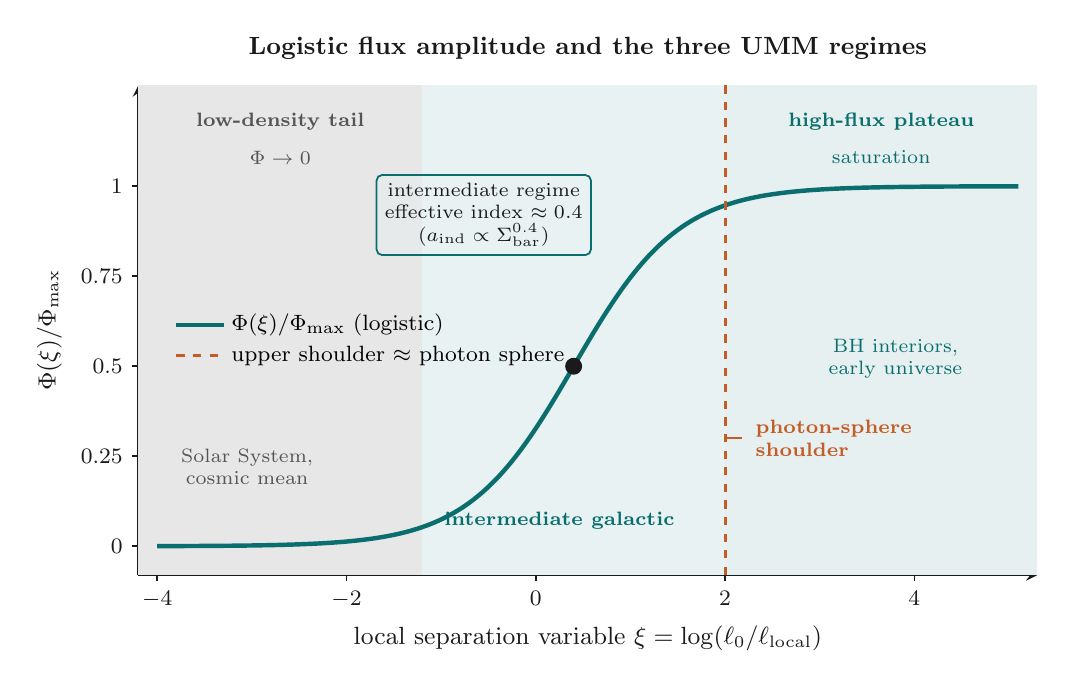
\begin{tikzpicture}
\begin{axis}[
  umm axis,
  width=13.0cm,
  height=7.8cm,
  xlabel={local separation variable $\xi=\log(\ell_0/\ell_{\mathrm{local}})$},
  ylabel={$\Phi(\xi)/\Phi_{\max}$},
  xmin=-4.2, xmax=5.3,
  ymin=-0.08, ymax=1.28,
  xtick={-4,-2,0,2,4},
  ytick={0,0.25,0.5,0.75,1.0},
  legend style={
    at={(0.03,0.48)},
    anchor=west,
    font=\footnotesize,
    draw=none,
    fill=none,
    cells={anchor=west},
  },
  title={Logistic flux amplitude and the three UMM regimes},
]
  % Regime background bands (drawn first so curve sits on top)
  \fill[ummLightGray!28] (axis cs:-4.2,-0.08) rectangle (axis cs:-1.2,1.28);
  \fill[ummFill] (axis cs:-1.2,-0.08) rectangle (axis cs:2.0,1.28);
  \fill[ummAccent!10] (axis cs:2.0,-0.08) rectangle (axis cs:5.3,1.28);

  % Logistic: alpha=1.8, xi_c = 0.4
  \addplot[ummAccent, line width=1.6pt, domain=-4:5.1, samples=200]
    {1/(1+exp(-1.8*(x-0.4)))};
  \addlegendentry{$\Phi(\xi)/\Phi_{\max}$ (logistic)}

  % Photon-sphere shoulder marker
  \draw[ummGas, line width=1.1pt, dashed]
    (axis cs:2.0,-0.08) -- (axis cs:2.0,1.28);
  \addlegendimage{line legend, ummGas, dashed, line width=1.1pt}
  \addlegendentry{upper shoulder $\approx$ photon sphere}

  % Midpoint marker
  \addplot[only marks, mark=*, mark size=2.4pt, ummDark, forget plot]
    coordinates {(0.4,0.5)};

  % Regime titles (top of each band) — no boxes
  \node[font=\scriptsize\bfseries, ummGray] at (axis cs:-2.7,1.18)
    {low-density tail};
  \node[font=\scriptsize, ummGray] at (axis cs:-2.7,1.08)
    {$\Phi\to 0$};

  \node[font=\scriptsize\bfseries, ummAccent] at (axis cs:0.25,0.07)
    {intermediate galactic};

  \node[font=\scriptsize\bfseries, ummAccent] at (axis cs:3.65,1.18)
    {high-flux plateau};
  \node[font=\scriptsize, ummAccent] at (axis cs:3.65,1.08)
    {saturation};

  % Photon-sphere label: horizontal, to the right of the dashed line (not on it)
  \draw[ummGas, line width=0.7pt]
    (axis cs:2.0,0.30) -- (axis cs:2.18,0.30);
  \node[font=\scriptsize\bfseries, ummGas, anchor=west, align=left]
    at (axis cs:2.22,0.30) {photon-sphere\\shoulder};

  % Intermediate index: very light semi-transparent fill, above flat part of left band
  % Positioned left of the steep rise so it does not cover the curve
  \node[font=\scriptsize, ummDark, align=center,
        draw=ummAccent, line width=0.65pt, rounded corners=2pt,
        fill=ummFill, fill opacity=0.30, text opacity=1,
        inner sep=3pt]
    at (axis cs:-0.55,0.92)
    {intermediate regime\\effective index $\approx 0.4$\\
     ($a_{\mathrm{ind}}\propto\Sigma_{\mathrm{bar}}^{0.4}$)};

  % Anchors (clear of curve)
  \node[font=\scriptsize, ummGray, align=center] at (axis cs:-3.05,0.22)
    {Solar System,\\cosmic mean};
  \node[font=\scriptsize, ummAccent, align=center] at (axis cs:3.8,0.52)
    {BH interiors,\\early universe};
\end{axis}
\end{tikzpicture}
\end{document}
